\section{Background}
    \begin{figure*}
        \centering
        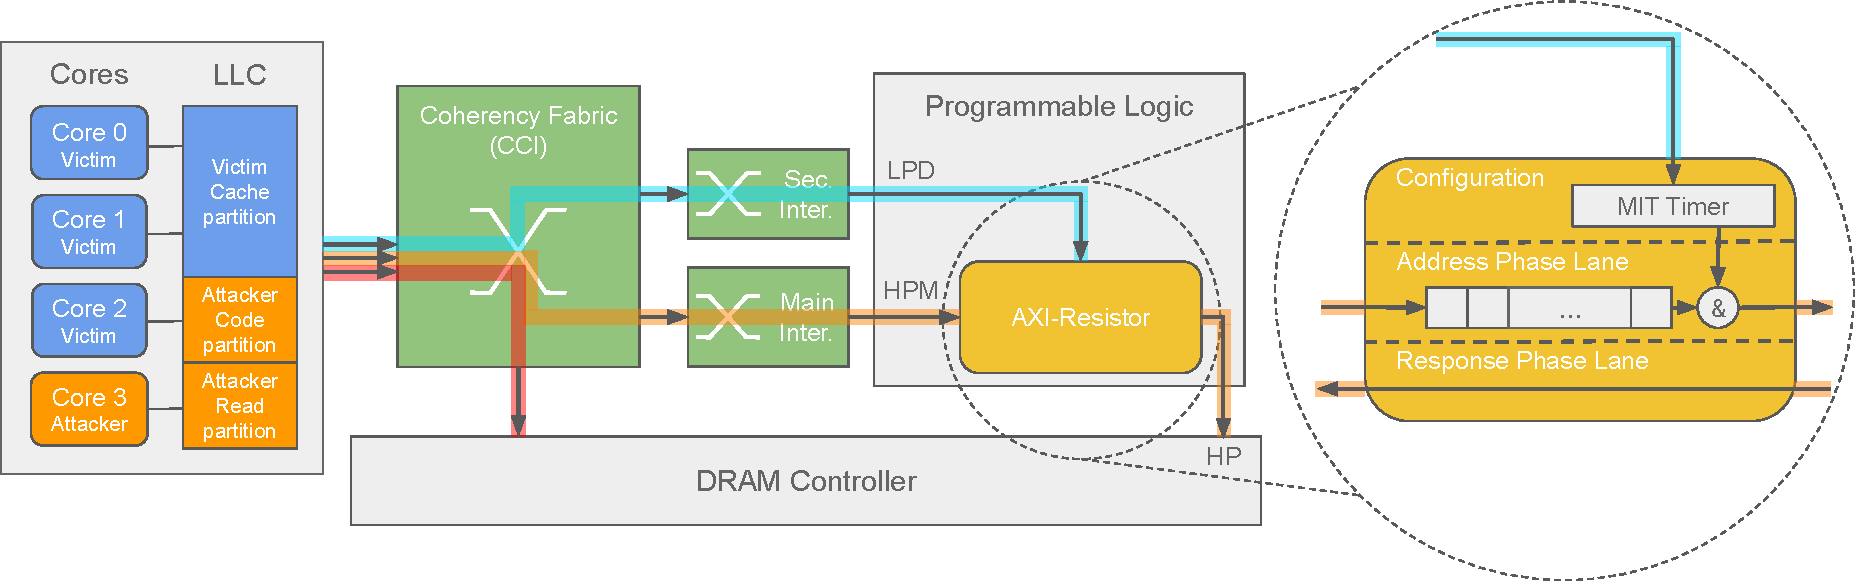
\includegraphics[scale=0.5]{images/Evaluation_setup.pdf}
        \caption{Schematic view of the considered setup with the partitioning of the core cluster (both cores and LLC) on the left, the different path taken by the transactions highlighted in cyan, orange and red, and the AXI-Regulator on the right.}
%        \caption{Schematic view of the system model with the partitioned core cluster, the different routes and the AXI-Resistor.}
        \label{fig:system_schematic}
    \end{figure*}
    \subsection{Non-blocking Caches}
%        Caches in modern MPSoCs are a crucial component that efficiently bridges the gap between the speed of the execution units and the main memory.
%        However, as good as they are at providing high bandwidth, \emph{blocking caches} are ineffective at hiding cache-miss penaty because they stall the execution units until the data is received from the main memory.
%        In order to hide this penalty and improve the cache performance, \cite{Kroft} proposed the first \emph{Miss-Handling-Architecture} (MHA).
%        This type of cache referred to as \emph{Non-blocking} relies on the introduction of a set of new registers called \emph{Miss Status Holding Register} (MSHR), which are in charge of tracking the status of cache line misses.
%        Each MSHR stores important information regarding the cache-miss such as the target address and the location of the cache line to refill.
%        For each level of cache in a system, the amount of MSHRs denotes the number of outstanding (i.e. simultaneous) transactions it can handle.
%        %This amount is known as the \emph{Memory-Level-Parallelism} (MLP).
%
%        At run time, a non-blocking cache behaves as follows. When a cache-miss occurs, the metadata of the cache-miss is stored in one of the available MSHRs. In case the same cache-miss already occurred and one MSHR already holds the metadata, the two requests are merged.
%        It is only once the cache line refill request has been served and placed in the proper cache line that the MSHR is made available to store new cache-misses requests.
%        Provided that all the MSHRs are used at a given instant, the system stops until one of them becomes available.

    Caches in modern MPSoCs are crucial components that efficiently circumvent the performance gap between the speed of the processing elements and the main memory.
    However, as good as they are at providing high bandwidth, \emph{blocking caches} are ineffective at hiding cache-miss penalty because they stall the processing elements until the data is received from the main memory.
    In order to hide this penalty and improve the cache performance, \cite{Kroft} proposed the first \emph{Miss-Handling-Architecture} (MHA).
    This type of cache referred to as \emph{Non-blocking} relies on the introduction of a set of new registers called \emph{Miss-Status-Holding-Register} (MSHR), which are in charge of tracking the status of cache line misses.
    Each MSHR stores important information regarding the cache-misses such as the target address and the location of the cache line to refill.
    For each level of cache in a system, the amount of MSHRs denotes the number of outstanding (i.e., simultaneous) transactions it can handle.
    This amount is known as the \emph{Memory-Level-Parallelism} (MLP).

    At run time, a non-blocking cache behaves as follows.
    When a cache-miss occurs, the metadata of the cache-miss is stored in one of the available MSHRs.
    In case the same cache-miss already happened and one MSHR already holds the metadata, the two requests are merged.
    It is only once the cache line refill request has been served and placed in the proper cache line that the MSHR is made available to store new cache-misses requests.
    If none of the MSHRs are available, the system stops until one of them becomes available.

    \subsection{Programmable Logic In the Middle (PLIM)}
%        The \emph{Programmable Logic In the Middle} (PLIM) is a new paradigm introduced by \cite{PLIM20} that takes advantage of the newly available platforms associating a traditional \emph{Processing System} (PS side) with a tightly integrated Programmable Logic (PL side).
%        In a system using PLIM, the PL side is leveraged such that the latter is located in between the core cluster and the main memory in the data path.
%        In other words, a PLIM module is a piece of custom logic located on the PL side that is capable of manipulating the transactions coming from the core cluster before they reach the main memory.
%        For instance, \cite{PLIM20} tackled important constraints imposed by the cache coloring technique by using a PLIM module (called \emph{bleacher}) by applying a configurable transformation on each incoming transaction address.
%        The use of a PLIM module broadens considerably the control over memory operations as it becomes possible to manipulate the memory traffic generated by the core cluster at the granularity of individual transactions.

%        The \emph{Programmable Logic In the Middle} (PLIM) is a new paradigm introduced by \cite{PLIM20} that takes advantage of the newly available platforms associating a traditional \emph{Processing System} (PS side) with a tightly integrated Programmable Logic (PL side).
%        In a PLIM system, the PL side is used as an intermediate step in the data path, located between the core cluster and the main memory.
%        Through this rerouting of the core cluster traffic, a PLIM module is a piece of custom logic located on the PL side that is capable of manipulating the transactions coming from the core cluster before they reach the main memory.
%        For instance, \cite{PLIM20} tackles significant constraints imposed by the cache coloring technique by using a PLIM module (called \emph{bleacher}) by applying a configurable transformation on each incoming transaction address.
%        Using a PLIM module broadens the control over memory operations considerably as it becomes possible to manipulate the memory traffic generated by the core cluster at the granularity of individual transactions.

    The \emph{Programmable Logic In the Middle} (PLIM) is a new paradigm introduced by \cite{PLIM20} that takes advantage of the newly available platforms associating a traditional \emph{Processing System} (PS side) with a tightly integrated Programmable Logic (PL side).
    In a PLIM system, the PL side is leveraged to create a secondary route between the core cluster and the main memory as displayed in Figure \ref{fig:system_schematic} with the orange route.
    This secondary route is populated with custom logic IPs, called PLIM modules, allowing the CPU-originated traffic to be manipulated before reaching the main memory.
    Despite the inherent cost of re-routing the traffic through the PL side, the use of PLIM modules broadens the control over memory operations considerably as it becomes possible to manipulate the memory traffic at the granularity of individual transactions.
    For instance, \cite{PLIM20} tackles significant constraints imposed by the cache coloring technique via a PLIM module, called \emph{bleacher}, which applies a configurable transformation on each incoming transaction address.

    In this paper, the PLIM paradigm is used to have fine control over certain transactions and as a mean to showcase the CPU-brainfreeze.
